\documentclass{article}
\usepackage[UTF8]{ctex}
\usepackage{pythonhighlight}

% Language setting
% Replace `english' with e.g. `spanish' to change the document language
\usepackage[english]{babel}
\usepackage{float}
% Set page size and margins
% Replace `letterpaper' with `a4paper' for UK/EU standard size
\usepackage[letterpaper,top=2cm,bottom=2cm,left=3cm,right=3cm,marginparwidth=1.75cm]{geometry}

% Useful packages
\usepackage{amsmath}
\usepackage{graphicx}
\usepackage[colorlinks=true, allcolors=blue]{hyperref}

\title{进度汇报3}
\author{雷远航}

\begin{document}

\maketitle

\begin{abstract}
第三次进度汇报

\end{abstract}

\section*{一:学习总结}
在之前所学习内容的基础上我又进一步学习了Image Alignment and Stitching、Structure from Motion、Depth Estimation、3D Reconstruction部分的理论知识,
主要对基本理论和基本方法有了一定的认识.同时,我也深度学习部分进行了一些初步的了解,并且根据pytorch的官方文档和Youtube上的教学视频对pytorch的使用进行了一些学习.

之后我计划对三维重建部分的知识和算法进行更近一步的学习,同时也学习一下计算机摄影学的部分.

\subsection*{Image Alignment and Stitching}
在这一部分我主要学习了进行图像对齐以及拼接的方法,基于特征检测和匹配的方法寻找对应的关键点,求解出图片之间的Projective Transformation矩阵,这种变换依赖于
几次拍摄时数字摄像机的不同参数以及多次拍摄之间摄像机的旋转和平移的关系.用RANSAC的方法进行Outliers的处理,在拼接时要对重叠交叉的部分进行处理.
这一部分我进行了一些简单的代码实现.
\begin{figure}[H]
    \centering
    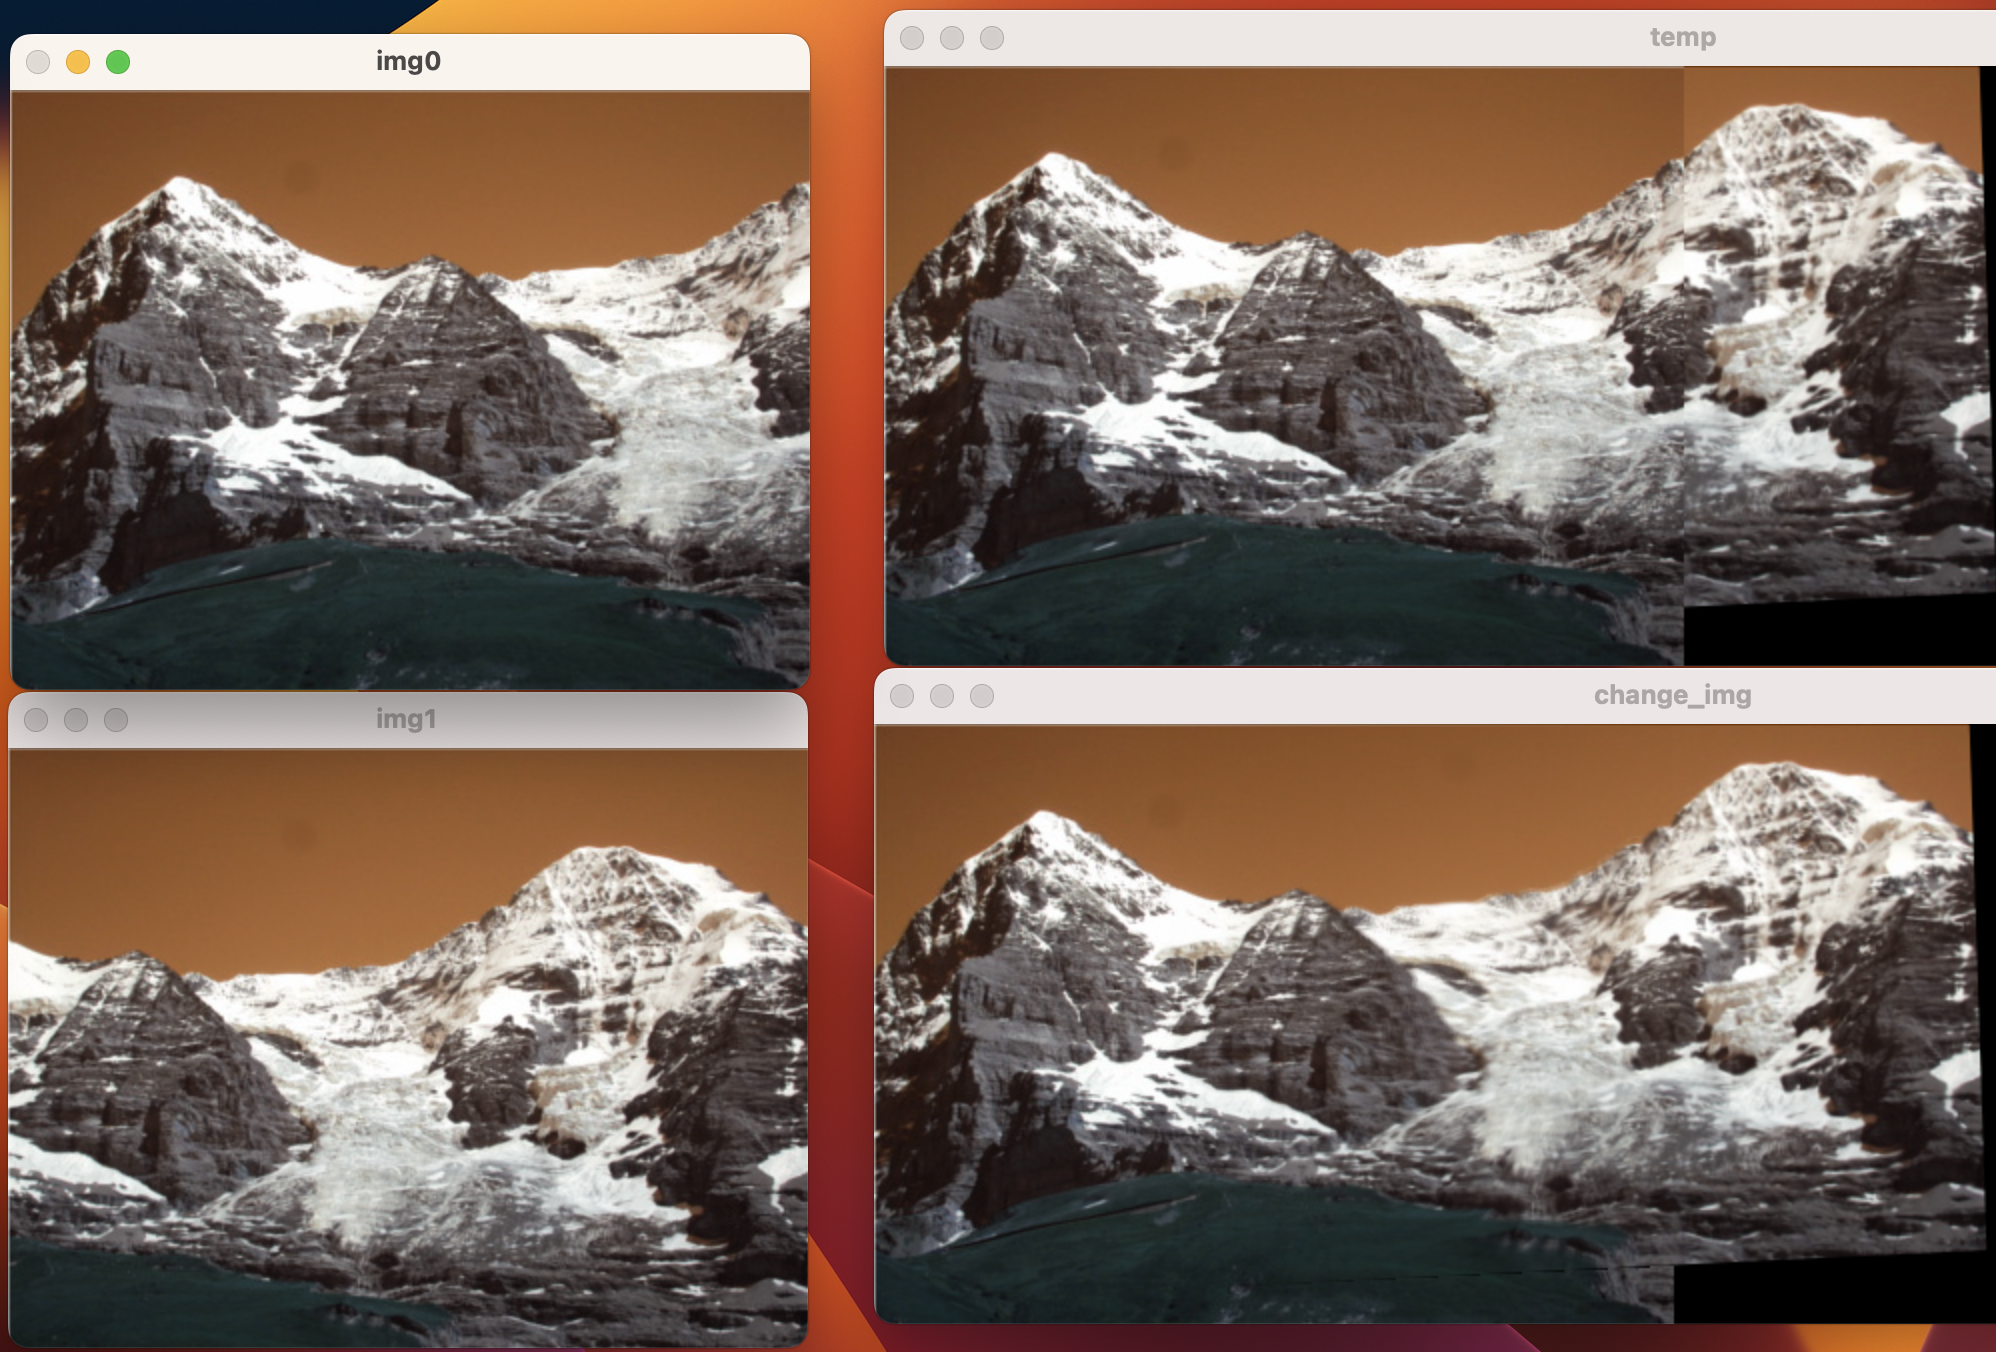
\includegraphics[width=0.8\textwidth]{2.png}
    \end{figure}



\subsection*{Structure from Motion}
这一部分我主要学习了从动态的视频或多组图像恢复出物体三维结构的流程,首先是摄像机内参、外参的标定,三维物体投影成为图像都基于摄像机的矩阵变换,同时
要考虑到相机畸变的问题.接着是对两组摄像机的图像的三角化矩阵变换关系,在深度图处理时也需要利用到这一三角化关系建立矩阵变换的方程,最后通过图像数据计算出三维空间的位置进行复原.

\subsection*{Depth Estimation、3D Reconstruction}
深度图的获取是进行三维重建的前提,通过双图的三角化关系可以进行深度的计算,在双目视觉的部分我主要看了一些视差的分析,以及在两个图像匹配过程的局部误差的分析,
利用多视图可以进行三维重建的工作,三维模型可以通过Point cloud、Occupancy、Signed distance、Mesh进行表示.这一部分我主要理解了三维重建的整体的工作流程.
同时我尝试使用了一下Colmap.
\begin{figure}[H]
    \centering
    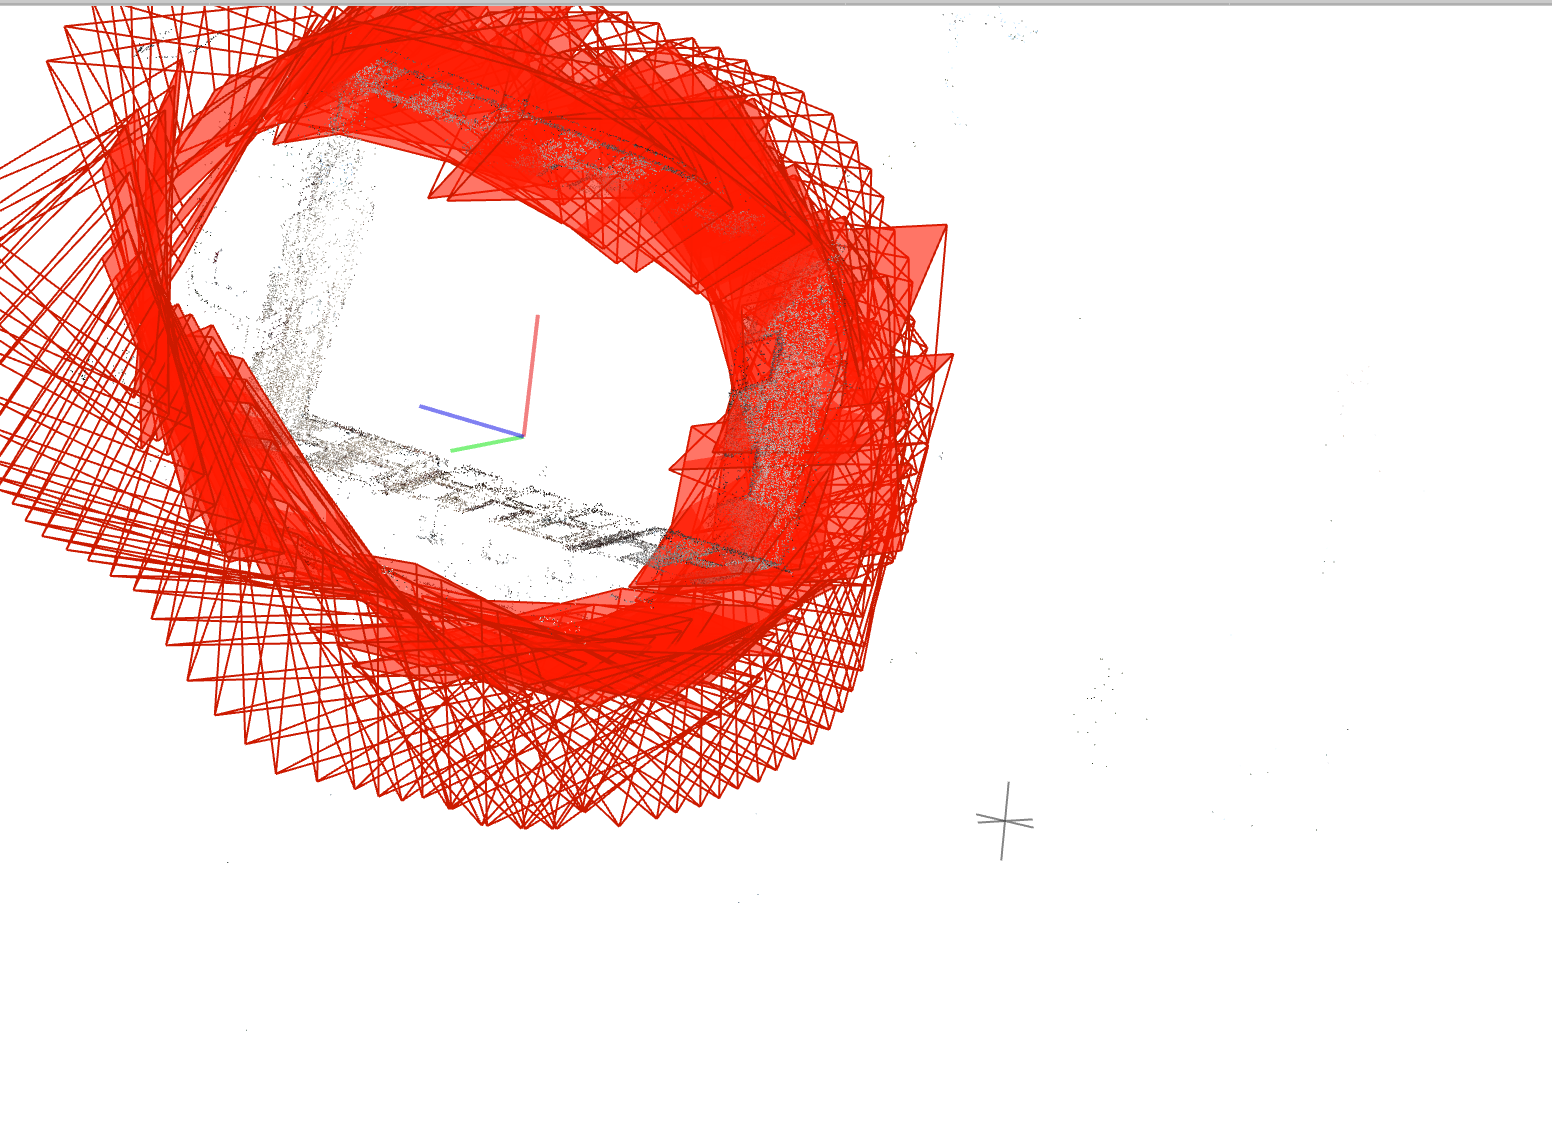
\includegraphics[width=0.8\textwidth]{1.png}
    \end{figure}


\subsection*{Pytorch}
我对Linear classifer、Neural networks、Convolutional neural networks、Training neural networks的原理和流程进行了学习,
使用pytorch建立简单的神经网络,训练数据实现图像分类器的流程进行了简单的实现.


\section*{二:一些提问}

1)目前我主要对基本概念和方法进行了一些学习,对整体的流程有了一定的认识,但进行的代码实现和算法的复现还比较少,后面计划对书上的部分习题进行实现,但我感觉书后的一些任务的描述比较简略有一些也比较抽象
请问是否有相关方面的一些其他具体任务的布置? 另外,对于深度学习部分我计划对cs231n课程网站上的lab进行完成来进一步加深学习.

\href{https://cs231n.github.io/assignments2022/assignment1/}{lab1 🔗}
\href{https://cs231n.github.io/assignments2022/assignment2/}{lab2 🔗}
\href{https://cs231n.github.io/assignments2022/assignment3/}{lab3 🔗}



2)我在尝试使用colmap和pytorch运行时自己的设备运行起来要花费较长的时间,如果后续使用需要的话是否会有GPU服务器资源的提供

3)在我所看到的一些关于深度神经网络的介绍中,我觉得整体的工作流程对参数的调整和试探有较多的依赖,至于为何选取、调整这些参数似乎并没有一个
很好的解释,是否这些调参的过程会有一些玄学因素在里面?

4)Image Alignment and Stitching、Structure from Motion、Depth Estimation、3D Reconstruction这些内容都对前面的特征检测和匹配的
工作有较多的依赖,在上一次的讨论中,如果图像中有金属的表面,那么如果有一些高光打在物体表面上,会导致一些视角下的纹理不可见,对匹配的过程造成困难.以及,
在不同视角下光线会有所不同,会导致错误的匹配.

如果场景中有镜子的话,镜中的像和实际的物体可能会产生错误的匹配.

除此之外如果图像中的物体的没有表面纹理,表面比较平滑也会对图像的匹配和重建造成较大的困难.

以及在通过运动图像复原三维结构时,如果物体有较大的运动幅度会使得匹配的过程较为困难,从而增大了三维重建时的难度.同时物体的遮挡、图像的分辨率较低等也是需要解决的问题.


\end{document}